\newpage
\chapter{Badania}
%\textbf{Przerzucone z wcześniejszych rozdziałów:}
%\begin{itemize}
%\item W przypadku wszystkich opisanych w tym rozdziale algorytmów za \emph{warunkiem stopu} można rozumieć wykonanie z góry określonej maksymalnej liczby iteracji pętli lub brak poprawy najlepszego rozwiązania w pewnej liczbie ostatnich przebiegów algorytmu. 
%\item Do ustawiana elitismu w genetycznym i memetycznym - Tak również postąpiono w trakcie przeprowadzania badań w ramach tej pracy - wykorzystano domyślny w pakiecie \emph{GA} rozmiar grupy chronionych osobników wynoszący 5\% populacji.
%\end{itemize}


\section{Specyfikacja funkcji testowych}
Znajdowanie coraz lepszych metod rozwiązywania problemów optymalizacyjnych oraz ich testowanie jest zagadnieniem na tyle powszechnym, że powstały w tym celu narzędzia to ułatwiające. Dzięki ujednoliceniu sposobu badań wydajności algorytmów możliwe jest porównywanie ich na płaszczyźnie tych samych problemów. Jednym z pakietów języka \emph{R} powstałym w tym celu jest \emph{globalOptTests} \cite{globalOptTestsPackage}. Stanowi go zbiór kilkunastu funkcji o różnej liczbie parametrów. Każda z nich dodatkowo opisana jest dziedziną wartości poszczególnych argumentów oraz wartością funkcji w ekstremum. Wszystkie problemy zawarte w pakiecie są zadaniami znalezienia \emph{minimum} globalnego.
\par
Na potrzeby przeprowadzenia badań porównawczych różnych algorytmów wybrano z pakiety \emph{globalOptTests} 3 funkcje, które zostaną opisane poniżej. Reprezentują one problemy  optymalizacyjne o różnej wymiarowości. 
\subsection{Funkcja Schaffer nr 2}
%\begin{itemize}
%\item wzor
%\item wykres, bo 2D
%\item dziedzina argumentow
%\item optimum: 0, w początku układu współrzędnych
%\item cechy: wiele ekstremow lokalnych zblizonych do optimum, ale odseparowanych. Większość dziedziny rozwiązań jest płaska jak stół 
%\end{itemize}

\par
Funkcja \emph{Schaffer nr 2} jest przedstawicielem rodziny funkcji multimodalnych dwuwymiarowych zaproponowanych przez autora w ramach pracy doktorskiej związanej między innymi z problemami optymalizacyjnymi \cite{schaffer1985some}. Cechuje się ona posiadaniem wielu ekstremów lokalnych o podobnych wartościach do optimum. Przebieg funkcji zaprezentowany na rysunku \ref{fig:Schaffer1} i opisywana jest wzorem \ref{eq:Schaffer1}. Poszukiwanym ekstremum jest minimum osiągane w początku układu współrzędnych przestrzeni rozwiązań \ref{eq:Schaffer1_optim}. Przeszukiwana przestrzeń rozwiązań stanowi płaszczyznę $\Re^2$ ograniczoną do przedziału \ref{eq:Schaffer1_range}.
\begin{equation} \label{eq:Schaffer1}
f(x)=0.5+\frac{\sin^2(x_1^2-x_2^2)-0.5}{[1+0.001(x_1^2+x_2^2)]^2}
\end{equation}
\begin{equation} \label{eq:Schaffer1_optim}
f(x)=0 \Leftrightarrow x_1,x_2=0
\end{equation}
\begin{equation} \label{eq:Schaffer1_range}
x_1,x_2\in[-120,100]
\end{equation}
\par
Dokonując przeglądu funkcji dostępnych w ramach pakietu \emph{globalOptTests} natrafiono na nieścisłość nazewniczą. Opisywana w tym miejscu funkcja nazywana przez autora oraz w literaturze mianem \emph{Schaffer nr 2} (lub \emph{Schaffer N.2}) przez autora pakietu została nazwana funkcją \emph{Schaffer1}. Fakt, iż przynajmniej jedna z funkcji pakietu opatrzona jest inną nazwą niż powinna sprawia, że przed wykorzystaniem dowolnej innej funkcji z pakietu powinno się najpierw zweryfikować, czy jej implementacja jest zgodna z opisem w literaturze.

\begin{figure} 
\centering
\begin{subfigure}{.5\textwidth}
  \centering
  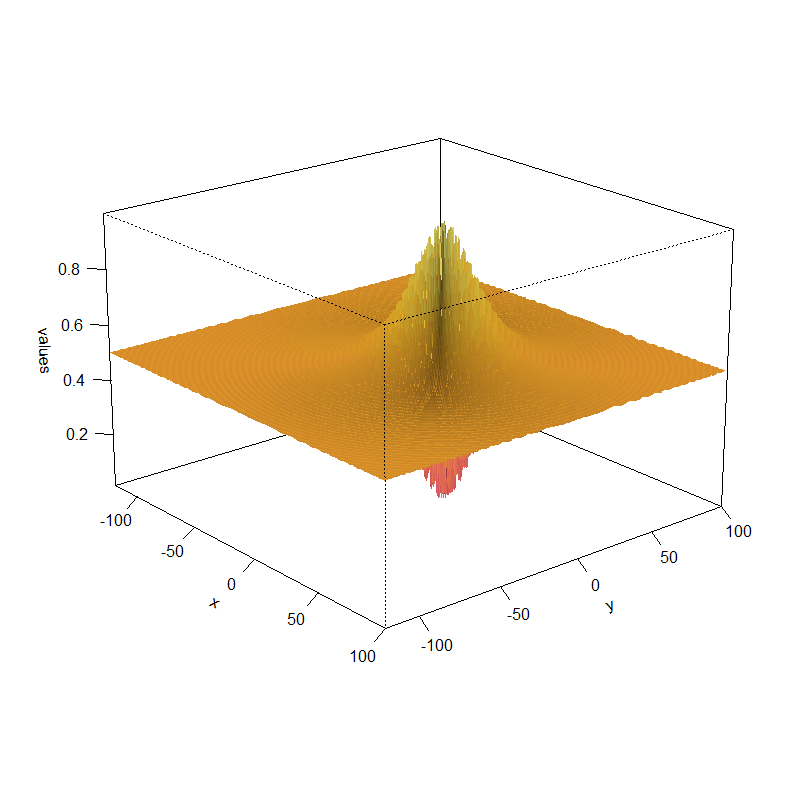
\includegraphics[width=\linewidth]{{img//roz03//Schaffer1_full_range.png}}
  \caption{ Pełna dziedzina argumentów}
  \label{fig:sub1}
\end{subfigure}%
\begin{subfigure}{.5\textwidth}
  \centering
  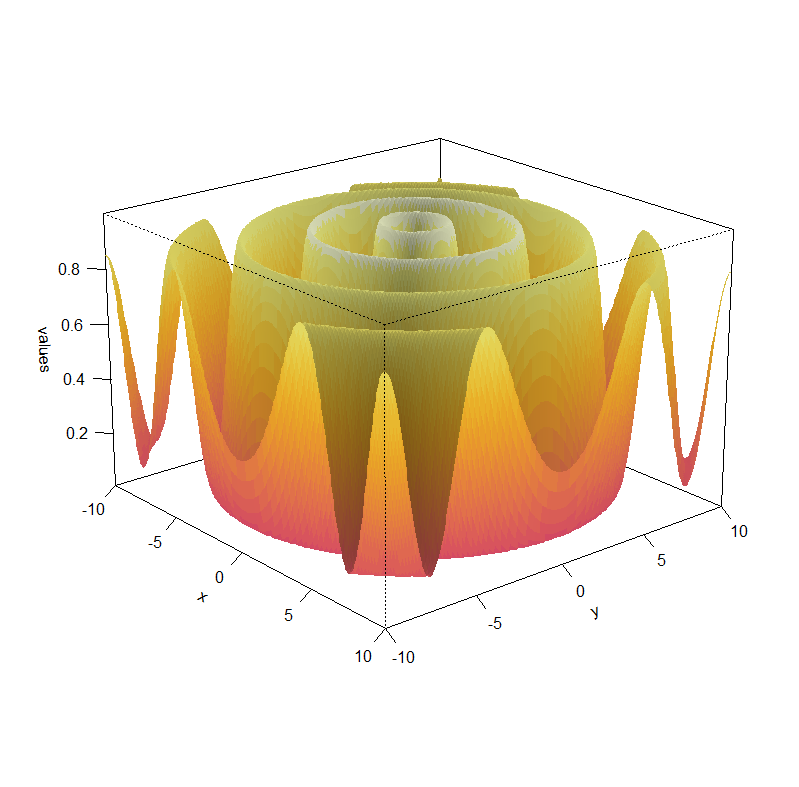
\includegraphics[width=\linewidth]{img//roz03//Schaffer1_small_range.png}
  \caption{Otoczenie optimum}
  \label{fig:sub2}
\end{subfigure}
\caption{Przebieg funkcji \emph{Schaffer nr 2}}
\label{fig:Schaffer1}
\end{figure}


\subsection{Funkcja Paviani}
%\begin{itemize}
%\item wzor
%\item dziedzina argumentow
%\item optimum: jakie i gdzie
%\item pewnie cos w necie ciekawego o nim jest
%\end{itemize}
\par
Drugą funkcją wykorzystaną w badaniach porównawczych jest funkcja \emph{Paviani}, która opisana jest wzorem \ref{eq:Paviani}. Została zaprezentowana w roli testowego problemu poddawanemu optymalizacji rzeczywistoliczbowej w ramach książki Davida Himmelblau'a \emph{Applied Nonlinear Programming} \cite{himmelblau1972applied}. Przestrzeń rozwiązań stanowi dziesięciowymiara przestrzeń ograniczona w przedziałach \ref{eq:Paviani_range}. Podobnie jak \emph{Schaffer nr 2} jest ciągła i różniczkowalna w całej dziedzinie argumentów. Nietypowy zakres wartości parametrów jest konsekwencją zbieżności funkcji do nieskończoności dla wartości $x=2$ i $x=10$. Jedyne oszukiwane minimum funkcji osiągane jest dla wartości \ref{eq:Paviani_optim}.
\begin{equation}\label{eq:Paviani}
f(x)=\sum_{i=1}^{10} \bigg(\log^2(x_i-2) + \log^2(10-x_i)\bigg) - \left(
\prod_{i=1}^{10} x_i\right)^{0.2}
\end{equation}
\begin{equation} \label{eq:Paviani_optim}
f(x)=-45.7784684040686 \Leftrightarrow x_i = 9.350266,\quad i = 1, ..., 10
\end{equation}
\begin{equation} \label{eq:Paviani_range}
x_i\in[2.0001,9.9999], \quad i=1,...,10
\end{equation}
\section{Opis środowiska testowego}
\begin{itemize}
\item parametry maszyny testowej

\end{itemize}


\section{Przyjęte miary efektywności algorytmów}
\label{sec:przyjete_miary_efektywnosci_algorytmow}
wszstko dla tych samych liczby iteracji
\begin{enumerate}
\item najlepsze znalezione rozwiązanie kolejno w iteracjach
\item średnie rozwiązanie populacji kolejno w iteracjach
\item czas osiągnięcia rozwiązań 90, 95 i 99%

\end{enumerate}
